%!TEX root = ../thesis.tex

\chapter{Umsetzung}
\label{chap:coding}
In diesem Kapitel wird auf den Aufbau der Implementierung eingegangen. Zunächst ein allgemeiner Überblick über das Vorgehen. Dies wird im folgenden als Pipeline bezeichnet und wird im \prettyref{sec:pipeline} allgemein erkläutert.

Nachdem ein genereller Überblick über die einzelnen Bestandteile gegeben wurde wird auf die einzelnen Schritte der Pipeline genauer eingegangen.
Anfänglich werden einmalige Vorbereitungsschritte aufgeschlüsselt, hierzu gehört zu einem großen Teil die Kalibrierung der genutzten Kamera in \prettyref{sec:camera} und die Bestimmung der Charakteristika dieser. 

Darauf folgt in \prettyref{sec:board} die Kalibrierung und die Erkennung der Felder des Dartboardes. Es werden verschiedene getestete Ansätze erörtert und ihre Vor- und Nachteile dargestellt.

Des Weiteren werden die einzelnen Abschnitte der Pipeline näher beleuchtet und auf die Implementierung und das Vorgehen eingegangen. Dies umfasst von der Segmentierung der Dinge, die nicht zum Dartboard gehören in \prettyref{sec:substraction}. Bis hin zur konkreten Bestimmung der erzielten Punktzahl in \prettyref{sec:score}. 
       
\section{Pipeline Überblick}
\label{sec:pipeline}
Ein genereller Überblick über die Pipeline wird in Abbildung \prettyref{Fig:pipeline} gegeben. Zu erkennen ist, dass es zwei sich wiederholende Teile gibt. Als Verbindungsglied zwischen diesen steht der Contour Storage. Dieser speichert Informationen zu jedem aufgenommenen Bild. Auf den Storage, seine Funktionsweise und die weitere Verarbeitung wird in \prettyref{sec:foreground} eingegangen. 

Es wird ein einmalig, zu beginn ausgeführter Teil aufgerufen, der die Kalibrierung, der Kamera übernimmt. Diese gehört nur bedingt zur Pipeline hinzu. Die Kamera Kalibrierung muss für eine spezifische Kamera nur ein einziges mal ausgeführt werden, abgesehen von dem Fall, dass die Kamera eine Fokussierung besitzt. In diesem Fall muss dieser Schritt nach jedem Fokus Vorgang erneut ausgeführt werden. Auf die Kalibrierung der Kamera wird im einzelnen in \prettyref{sec:camera} eingegangen.

Ist die generelle Kalibrierung abgeschlossen, können die hieraus gewonnenen Informationen genutzt werden, um das Dartboard und dessen Felder zu segmentieren und unterscheiden zu können. Das Resultat dieser Kalibrierung ist eine Funktion, die eine Abbildung von einem Pixel zu einer spezifischen Punktzahl auf dem Dartboard darstellt. In \prettyref{sec:board} wird genauer beschrieben, welche Ansätze zu diesem Zweck verfolgt wurden und wie die letztendliche Umsetzung vorgenommen wurde.

Diese beiden Schritte können übersprungen werden, sofern das Setup sich nicht verändert hat, und die Kalibrierungen in einer Datei, als JSON, gespeichert wurden und erneut geladen werden können. 
\begin{figure}
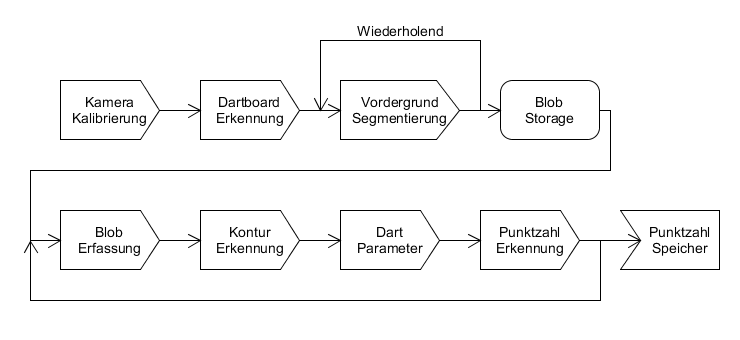
\includegraphics[width=\textwidth]{media/pipeline.png}\\
\caption{\textbf{Übersicht der einzelnen Schritte}}
\label{Fig:pipeline}
\end{figure}

Es werden zwei separate Threads gestartet. In der Abbildung ist der erste Thread grau markiert (Substrator) und der zweite türkis. Der Substractor dient dazu den Contour Storage mit Informationen zu füllen. In \prettyref{sec:substraction} wird das Vorgehen erläutert und welche Informationen bestimmt und gespeichert werden.
Der zweite Thread wird in mehrere Sub-Schritte unterteilt. 
Zunächst verwendet die Blob-Erfassung, mehr in \prettyref{sec:blob}, die Informationen im Storage um ein Bild zur weiteren Verarbeitung zu generieren. Die gewonnenen Informationen werden für die weitere Verarbeitung zu Kontur-Erkennung genutzt, nähere Beschreibung in \prettyref{sec:foreground}.

Abschließend werden die Dart-Parameter bestimmt und in der Punktzahl-Erkennung mithilfe der Bildpunkt-Punktzahl-Funktion in die erzielte Punktzahl überführt. Diese wird anschließend abgespeichert.


\section{Kamera Kalibrierung}
\label{sec:camera}
Im \prettyref{sec:camerageo} wurden bereits das Kamera Modell und die Parameter einer Kamera erläutert. So heißt es in \autocite[5]{Zhang2000} \textquote{Camera calibration is a necessary step in 3D computer vision in order to extract metric information from 2D images.} Nun gilt es eben diese Parameter zu bestimmen um genauere Daten aus den Bildern der Kamera zu erlangen. 

Diese Kalibrierung ist vorrangig dafür gedacht die intrinsischen Parameter der Kamera zu bestimmen. Die extrinsischen Parameter werden auf andere Art bestimmt, bzw. in einem anderen Schritt. Die Bestimmung der extrinsischen Parameter wird in \prettyref{sec:board} erläutert.

Es gibt mehrere verschiedene Möglichkeiten eine Kalibrierung der Kamera vorzunehmen. Diese sind: mit 3D-Objekten, mit 2D-Ebenen oder 1D-Linien. Dabei haben diese verschiedenen Varianten einen unterschiedlich hohen Aufwand, Genauigkeit und Komplexität in der Berechnung. 

So muss für jede dieser Varianten bestimmte Features und deren Position bekannt sein. Dies ist bei einem 3D-Objekt schwieriger zu bestimmen, als bei einer Ebene. Daher wurde der Einfachheit halber auf die Ebene zurückgegriffen. 
\begin{figure}
\subfloat[Schachbrettmsuter]{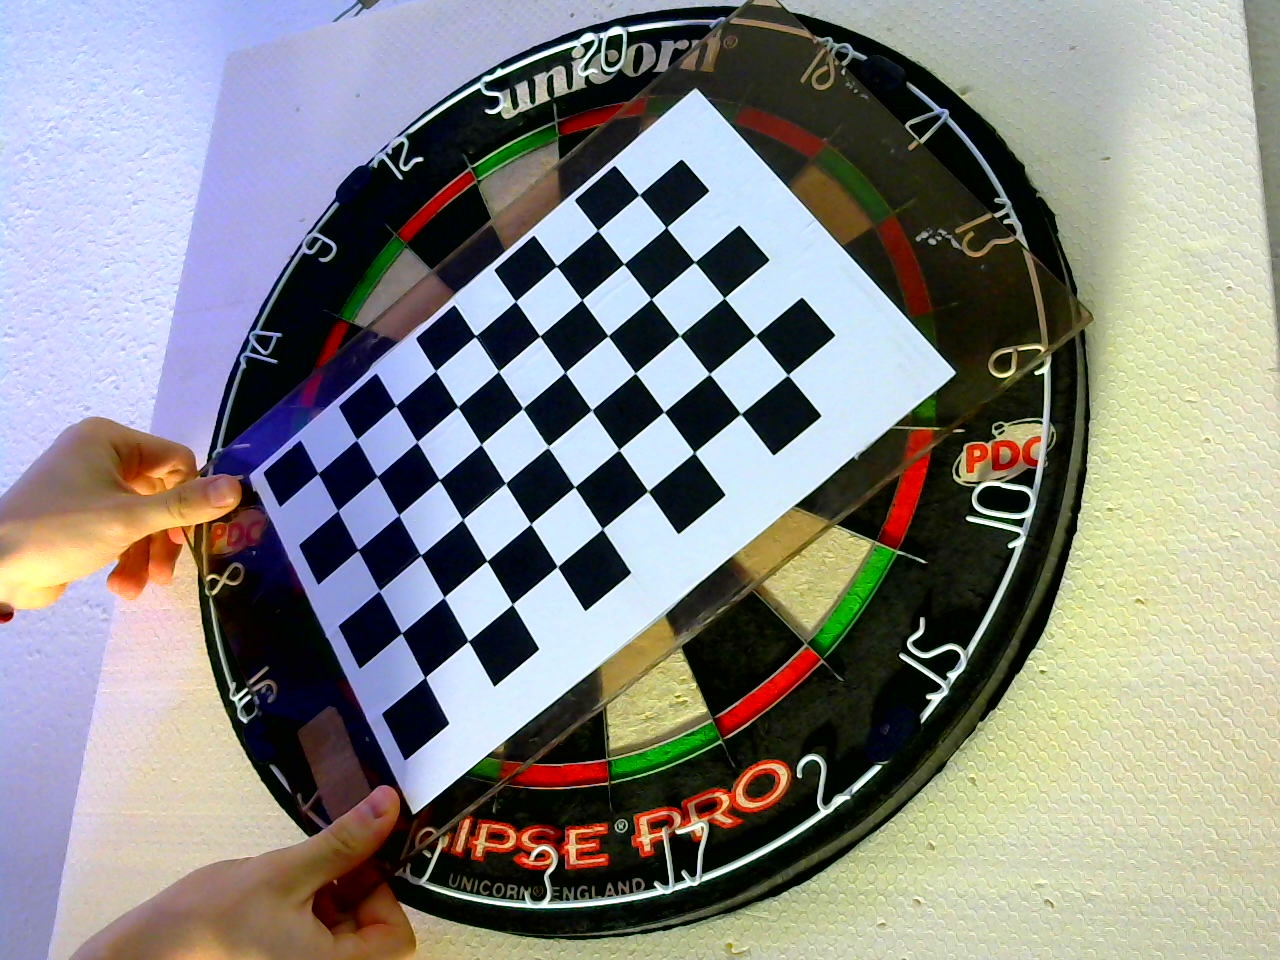
\includegraphics[width=0.5\textwidth]{media/calibraw1.jpg}}\qquad
\subfloat[Muster mit erkannten Punkten]{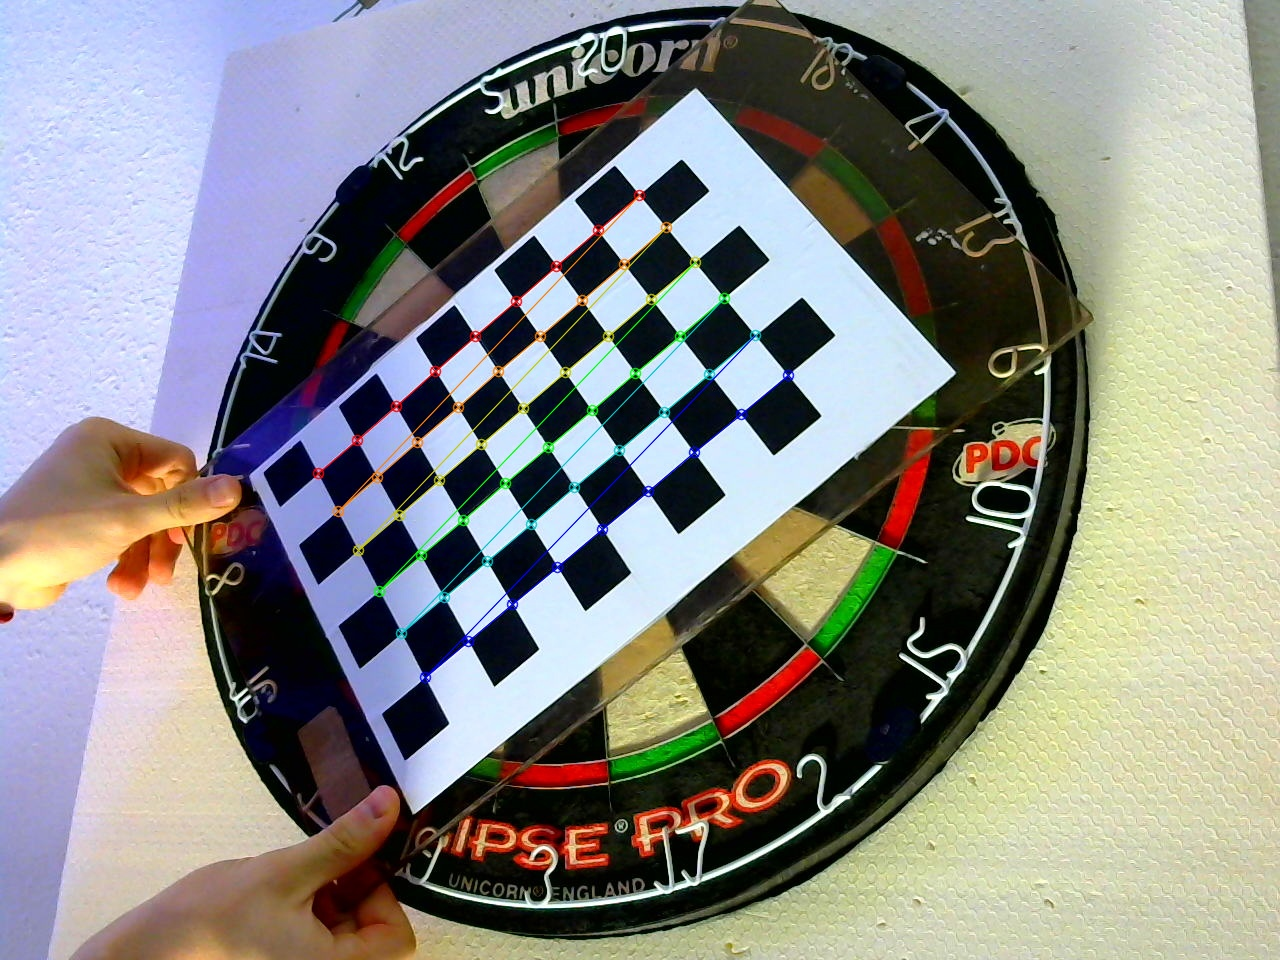
\includegraphics[width=0.5\textwidth]{media/calibrated1.jpg}\\}
\caption{\textbf{Eines der zur Kalibrierung genutzten Bilder}}
\label{Fig:calibplane}

%\caption{\textbf{Erkannte Feature Punkte/Schnittpunkte}}
%\label{Fig:calibplanefeature}
\end{figure}
In Abbildung \prettyref{Fig:calibplane} ist auf der linken Seite eines der Bilder zu sehen, mit denen die zum Test der Implementierung genutzten Kamera kalibriert wurde. Dies ist ein Muster von $9x6$ Schnittpunkten. Auf der rechten Seite sind die erkannten Feature-Punkte eingezeichnet. Für dieses Schachbrettmuster ist der Abstand der einzelnen Schnittpunkte durch ausmessen bekannt und mit $26mm$ Abstand entlang der Graden voneinander gegeben. 

Wie bereits beschrieben wird OpenCV \prettyref{sec:opencv} zur Implementierung genutzt. OpenCV bietet einige Funktionen um die Kamera Kalibrierung durchzuführen. Die Dokumentation von OpenCV3 \autocite{Opencv3Camera2016} zeigt die dafür zur Verfügung gestellten Funktionen. 
\begin{lstlisting}[frame=single]
ret, corners = findChessboardCorners(image, patternSize) 
corners2 = cornerSubPix(image, corners, winSize, zeroZone,\\
               criteria) 
ret, mtx, dist, rvecs, tvecs = calibrateCamera(\\
               objectPoints, imagePoints, imageSize,\\
               cameraMatrix, distCoeffs[, rvecs[,\\
               tvecs[, flags[, criteria]]]]) 
newcameramtx, roi = getOptimalNewCameraMatrix(mtx, dist,\\
               imageSize, alpha , newimageSize)
\end{lstlisting}
So wird \textit{findChessboardCorners} verwendet um die Schnittpunkte im Schachbrettmuster zu erkennen und die dazugehörigen Koordinaten zu identifizieren. Hierzu wird eines der Bilder mit dem Schachbrettmuster in ein Graustufenbild gewandelt und der Funktion übergeben, zusätzlich wird die Größe des Schachbrettmusters übergeben $(9,6)$. Dies liefert zum einen den Erfolg der Funktion als Boolean zurück und zum anderen die Bildkoordinaten der gefundenen Schnittpunkte. 
Die gefundenen Koordinaten sind allerdings nur approximierte Werte, daher ist es empfehlenswert \textit{cornerSubPix} auf demselben Bild mit den bereits ermittelten Schnittpunkten aufzurufen. Diese dient der genaueren Bestimmung der Bildkoordinaten, um eine bessere Genauigkeit zu erreichen. Die Funktion gibt die neuen Koordinaten der Schnittpunkte zurück. 

Um die Parameter der Kamera zu errechnen werden die Bildpunkte, der Schachbrettschnittpunkte und die zugehörigen Objektpunkte benötigt. Die Objektpunkte sind in diesem Fall die Punkte auf dem Schachbrett. Es wird davon ausgegangen, dass sich die Punkte alle auf einer Ebene befinden \textit{z=0}. Die Objektpunkte sehen in etwa wie folgt aus: $[[0,0,0], [26,0,0],...,[0,26,0],[0,52,0],...,[234,156,0]]$

Da es einer Ungenauigkeit, durch Rauschen und andere Fehler kommen kann wird nicht nur ein Bild zur Kalibrierung genutzt, sondern mehrere. Um eine der Linien entlang des Schachbrettmusters zu bestimmen reichen in der Theorie zwei Punkte. Aus bereits genannten Gründen werden allerdings auch hier mehrere Punkte verwendet. Zudem wird kein quadratisches Schachbrett genutzt, da so die Orientierung des Musters erkannt werden kann. 
Der in OpenCV verwendete Algorithmus basiert auf der Arbeit von Zhengyou Zhang. In "`Emerging Topics in Computer Vision"' \autocite{Medioni:2004:ETC:993884} empfiehlt dieser: \textquote{(...), we recommend 4 or 5 different orientations for better quality.} \autocite[24]{Zhang2000}.

So werden zu mehreren Bildern, mit unterschiedlicher Orientierung des Schachbrettes zur Kamera, die Bildpunkte bestimmt und gespeichert. Diese werden anschließend gesammelt an die Funktion \textit{calibrateCamera} übergeben. \textit{criteria} enthält Informationen für den Berechnungsalgorithmus, wie zum Beispiel die Distanz zwischen zwei Schnittpunkten. Die weiteren Parameter der Funktion sind optional und dienen der genaueren Berechnung.
Die Funktion gibt fünf Dinge zurück: \textit{ret} ist ein Boolean, ob die Berechnung erfolgreich war, \textit{mtx} die Kameramatrix, die die intrinsischen Parameter der Kamera enthält, \textit{dist} die Verzerrungsparameter, \textit{rvecs} ein Rotationsvektor, der die Rotation zwischen Kamera und Schachbrettmuster wiedergibt und zuletzt \textit{tvecs} ein Translationsvektor, der die Translation zwischen Kamera und Schachbrettmuster wiedergibt. Dabei sind Rotations- und Translationsvektor nicht weiter von Interesse, da diese nicht die Relation zum Dartboard wiedergeben. Wie die hierfür nötigen Vektoren bestimmt werden wird in \prettyref{sec:board} erläutert. Ein Beispiel für eine Matrix mit der genutzten Kamera sieht wie folgt aus:
$A= 
\begin{bmatrix} 
1416.55 & 0.0 & 687.84 \\
0.0 & 1416.51 & 476.39 \\
0.0 & 0.0 & 1.0\end{bmatrix}$.

Damit der Kalibrierungsvorgang nicht zu jedem Start der Software durchgeführt werden muss, werden die gewonnenen Parameter als JSON-String in eine Datei geschrieben. Zur nächsten Ausführung der Software kann dieser wieder geladen werden. 


\section{Erkennung des Dartboards}
\label{sec:board}
%\begin{itemize}
%\item     mehrere Ansätze
%\item     Blobs des boardes erkennen
%\item     Felder Kanten erkennen
%\item     Board Kalibrieren als Erweiterung der Kamera Kalibrierung
%        
%\item        Dartboard Koordinaten bestimmen im Verhältnis zur Kamera. Eigentliche Kalibrierung via klicken,
%\item       wie viele Punkte sind nötig
%\end{itemize}
Im Laufe der Implementierung wurden verschiedene Ansätze getestet, um das Dartboard und die Felder zu erkennen. Einige der Ansätze wurden verworfen, da sie nicht  zum gewünschten Ergebnis führten. Dabei wurde bei allen Ansätzen grundsätzlich ein gemeinsames Vorgehen verfolgt. So wird kein vollautomatischer Ansatz verfolgt, sonder auf eine Kalibrierung durch den Nutzer zurückgegriffen. 

Im ersten Ansatz war die Grundidee, den farblichen Unterschied der Felder zu nutzen. So sind die einfachen Felder, entweder schwarz oder weiß. Zudem haben Doppel- und Tripplefelder bei weißen Feldern eine grüne Farbe und bei schwarzen eine rote Farbe. 
Jedes der Felder, des Dartboards hat also eine von 4 Farben. 

Der Nutzer wird via GUI gebeten jeweils bestimmte Felder im Bild anzuklicken. So kann nicht nur der tatsächliche Farbwert ermittelt werden, sondern auch die Position bestimmter Felder im Bild. Anhand der Information und des Wissens über die Anordnung der Felder eines Dartboards kann dann also bestimmt werden welches Feld sich relativ zu den angeklickten befindet. 
\begin{figure}[ht]
\subfloat[Ausgangsbild]{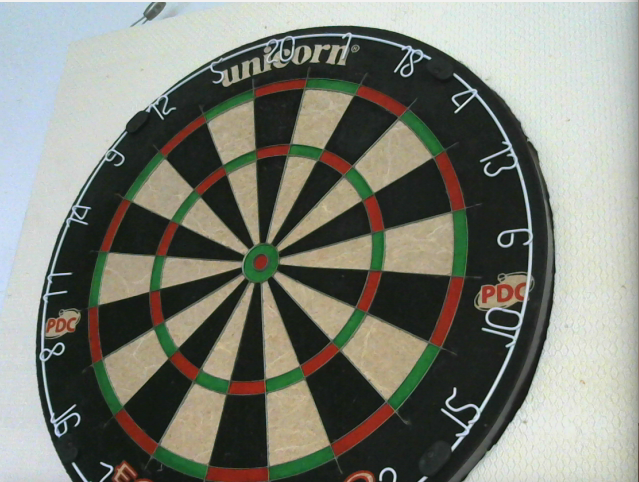
\includegraphics[width=0.48\textwidth]{media/undetected.png}}\qquad
\subfloat[grüne Felder]{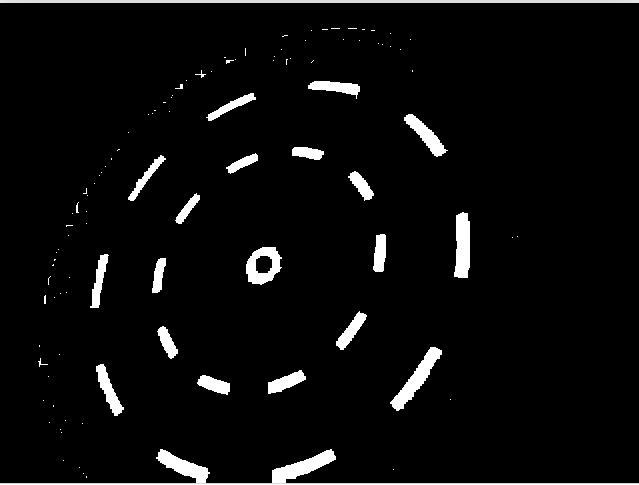
\includegraphics[width=0.48\textwidth]{media/greendetected.png}}\\
\subfloat[rote Felder]{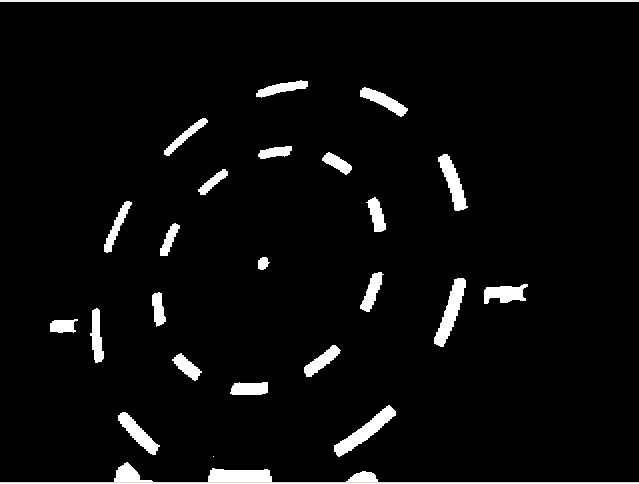
\includegraphics[width=0.48\textwidth]{media/reddetected.png}}\qquad
\subfloat[schwarze Felder]{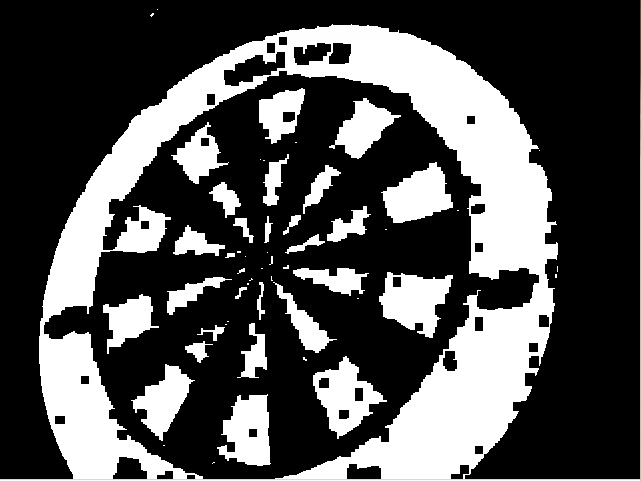
\includegraphics[width=0.48\textwidth]{media/blackdetected.png}}
\caption{\textbf{Ausgangsbild und verschiedene Farbfilter}}
\label{Fig:dartblobs}
\end{figure}
In Abbildung \prettyref{Fig:dartblobs} ist ein Beispiel dafür zu sehen. Hier wurde im Ausgangsbild ein grünes, ein rotes und ein schwarzes Feld ausgewählt. Nun ist bereits im Bild \textbf{(d)} eines der aufgetretenen Probleme zu erkennen. Bei schwarzen und weißen Feldern kann es durch farbliche Nähe und den nicht komplett einfarbigen Feldern zu Unschärfe und Rauschen kommen. Zudem können Schatten und andere widrige Lichtverhältnisse ebenfalls sehr störend sein, da in diesem Fall die Farbwerte gleicher Felder stark abweichen können. 
Zur Bestimmung wurde ein einfaches Tresholding auf dem Ausgangsbild gemacht. Also alle Pixel in einem bestimmten Farbbereich werden in ein neues Bild übertragen, in diesem Fall ein binär Bild. Auf diesem können dann Kontur-Erkennung und andere Algorithmen genutzt werden, um die zu einem Feld gehörigen Pixel zuzuordnen.


Aus dem Grund der Anfälligkeit und Ungenauigkeit wurde ein weiterer Ansatz getestet.
In diesem Ansatz wurde ebenfalls auf eine Interaktion mit dem Nutzer zurückgegriffen.
Hierbei wurde genutzt, dass die Ausmaße der Dartboards standardisiert sind. So kann ein Modell eines Dartboards implementiert werden. Dies entspricht einer Ebene, auf der die Schnittpunkte zwischen den Ringen und der Feldabgrenzung liegen. Abbildung \prettyref{Fig:dartmodel} wird dem Nutzer zur Kalibrierung angezeigt. Ausgegangen wird hier von einem Dartboard-Koordinatensystem, das den Ursprung in der Mitte des Boards hat.  
\begin{figure}
\centering
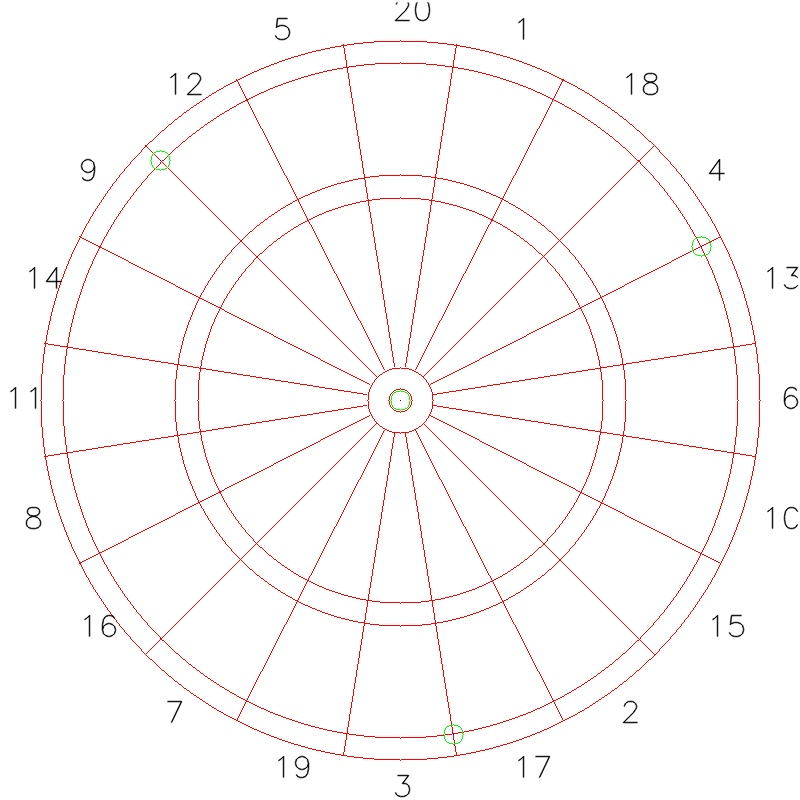
\includegraphics[width=0.5\textwidth]{media/confighints.jpg}\\
\caption{\textbf{Modell des Dartboards}}
\label{Fig:dartmodel}
\end{figure}
Die in der Abbildung markierten Punkte sollen vom Nutzer im Kamerabild markiert werden. 
Diese Punkte sind im Board-Koordinatensystem folgende:
$P_1 = \begin{bmatrix}0& 0& 0 \\\end{bmatrix}^\intercal 
P_2 = \begin{bmatrix}142.56& 72.64& 0 \\\end{bmatrix}^\intercal\\
P_3 = \begin{bmatrix}25.03& -158.03& 0 \\\end{bmatrix}^\intercal
P_4 = \begin{bmatrix}-113.14& 113.14& 0 \\\end{bmatrix}^\intercal$.
Zum einen wurde das Zentrum $(P_1)$ gewählt und zum anderen Punkte $P_2,P_3,P_4$ auf dem Dartboard verteilt. Mit Hilfe des Nutzers wird so eine Zuordnung zwischen den Objektpunkten und Bildpunkten erstellt. Parallel zur in \prettyref{sec:camera} erläuterten Kamera-Kalibrierung kann nun aus aus diesen beiden zueinander gehörigen Punkten eine Translations- und eine Rotationsmatrix errechnet werden. Hierbei wird auf die bereits abgeschlossene Bestimmung der intrinsischen Parameter der Kamera zurückgegriffen. Die bereits bestimmten Parameter werden genutzt und in der Berechnung der resultierenden Matrizen berücksichtigt. Hierbei wird die in OpenCV implementierte Funktion \textit{solvePnP(objectPoints, imagePoints, cameraMatrix, distCoeffs)} genutzt. Diese ermöglicht die Berechnung der Matrizen aus bereits aufgezählten Parametern. Übergeben werden:
\begin{itemize}
\item \textbf{objectPoints:} Punkte $P_1$ bis $P_4$ im Boardkoordinatensystem
\item \textbf{imagePoints:} Die Bildkoordinaten der vom Nutzer angeklickten Pixel
\item \textbf{cameraMatrix:} Intrinsische Parameter, entsprechend Matrix $A$ aus \prettyref{sec:camera}
\item \textbf{distCoeffs:} Verzerrungsparameter ebenfalls durch Kamerakalibrierung bestimmt 
\end{itemize}
Mithilfe dieser Matrizen, kann nun der zu einem Bildpunkt assoziierte Objektpunkt berechnet werden. Aus dem Objektpunkt kann dann Anhand des Modelles des Dartboards die Punktzahl ermittelt werden. 

Rückblickend auf die Kamera-Kalibrierung und in diesem Kapitel beschriebene Dartboard-Kalibrierung sind noch Optimierungen möglich. Aufgrund der bekannten Ausmaße des Dartboards könnte auch dessen Muster zur Bestimmung der intrinsischen Parameter der Kamera  genutzt werden. Dafür müssten im Idealfall alle Schnittpunkte zwischen Ringen und Feldlinien im Kamerabild erkannt und assoziiert werden können. Ein dabei aufgetretenes Problem ist, dass die Kanten nicht eindeutig erkannt werden können. Der Grund liegt in der Beschaffenheit des Dartboardes, so ist die Abgrenzung der Felder nicht scharf genug und besitzt eine gewisse Breite. Weiterführend wäre es also denkbar, dass die Schritte der Kamera- und Dartboard-Kalibrierung zusammengefasst würden. 



\section{Extraktion des Vordergrundes}
\label{sec:substraction}
Nachdem der Hintergrund, also das Dartboard erkannt und einem Modell zugeordnet wurde müssen nun die Darts selbst erkannt werden. Das Dartboard bildet dabei den statischen Hintergrund, während die Darts den sich verändernden Vordergrund des Bildes darstellen. 
In den bisherigen Abschnitten wurden einzelne Kamerabilder betrachtet. Im folgenden wird von einem Video, bzw. einem Live-Bild der Kamera ausgegangen.

Background-Substraction Algorithmen basieren auf einer gemeinsamen Idee.
Grundsätzlich werden dabei 3 Schritte angewandt:
\begin{enumerate}
\item Hintergrundmodell erstellen \textit{Abbildung (\prettyref{Fig:background} a)}
\item Aktuelles Bilder mit dem Modell vergleichen, bzw. Hintergrund von dem Modell abziehen \textit{(Abbildung \prettyref{Fig:background} b)}
\item Daten eventuell nachbearbeiten
\item Vordergrund-Maske ausgeben \textit{(Abbildung \prettyref{Fig:background} c)}
\item Schritt 2.
\end{enumerate}
Hierbei ist der 3. Schritt eine optionale Möglichkeit um das Ergebnis zu verbessern. 
Der 5. Schritt soll dabei nur andeuten, dass sich das Vorgehen für jedes neue Bild, des Videos bzw. Live-Bilder wiederholt wird.
\begin{figure}[ht]
\subfloat[Hintergrund]{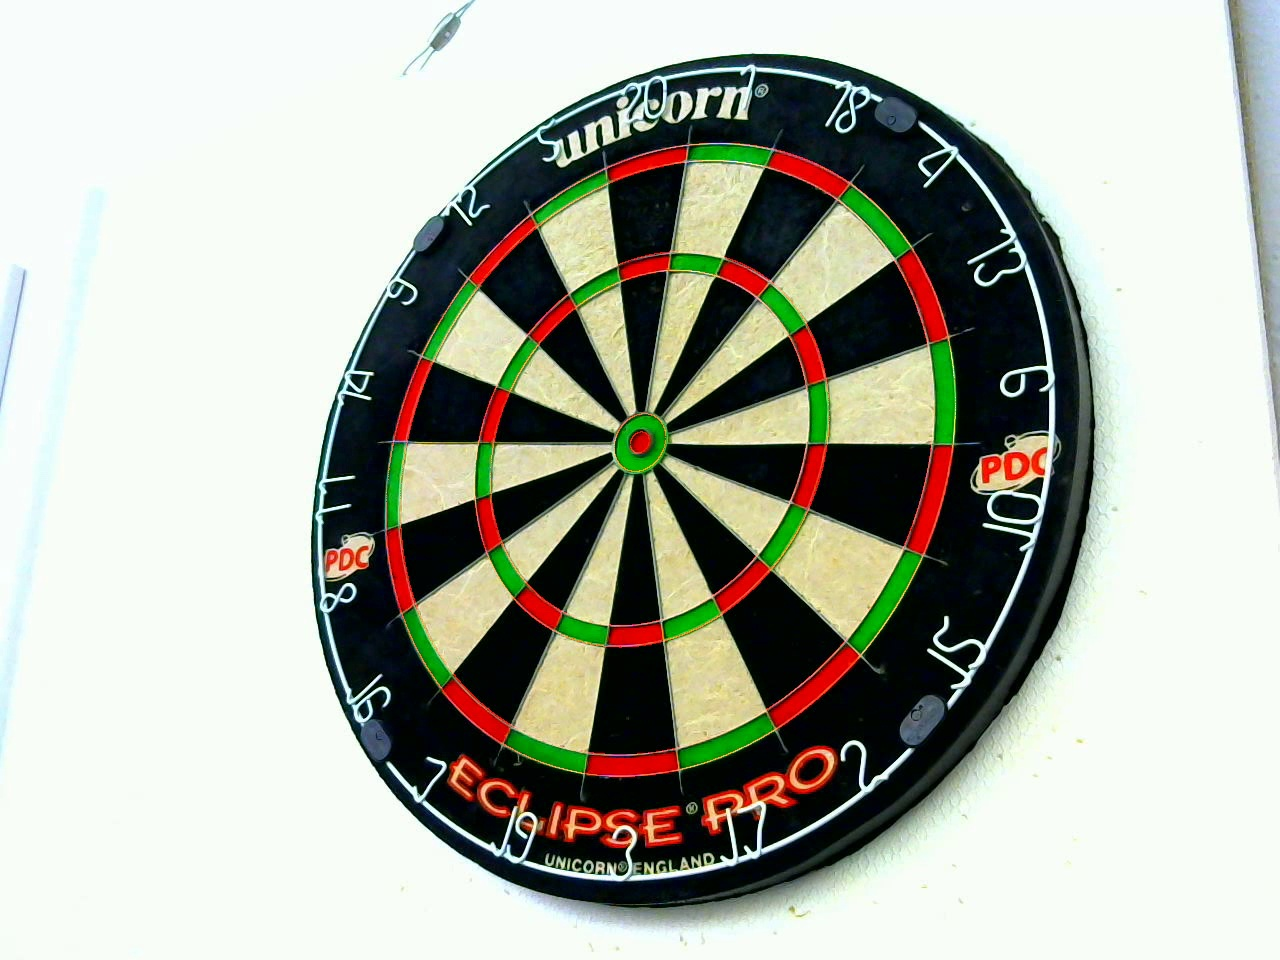
\includegraphics[width=0.48\textwidth]{media/background}}\qquad
\subfloat[Aktuelles Bild]{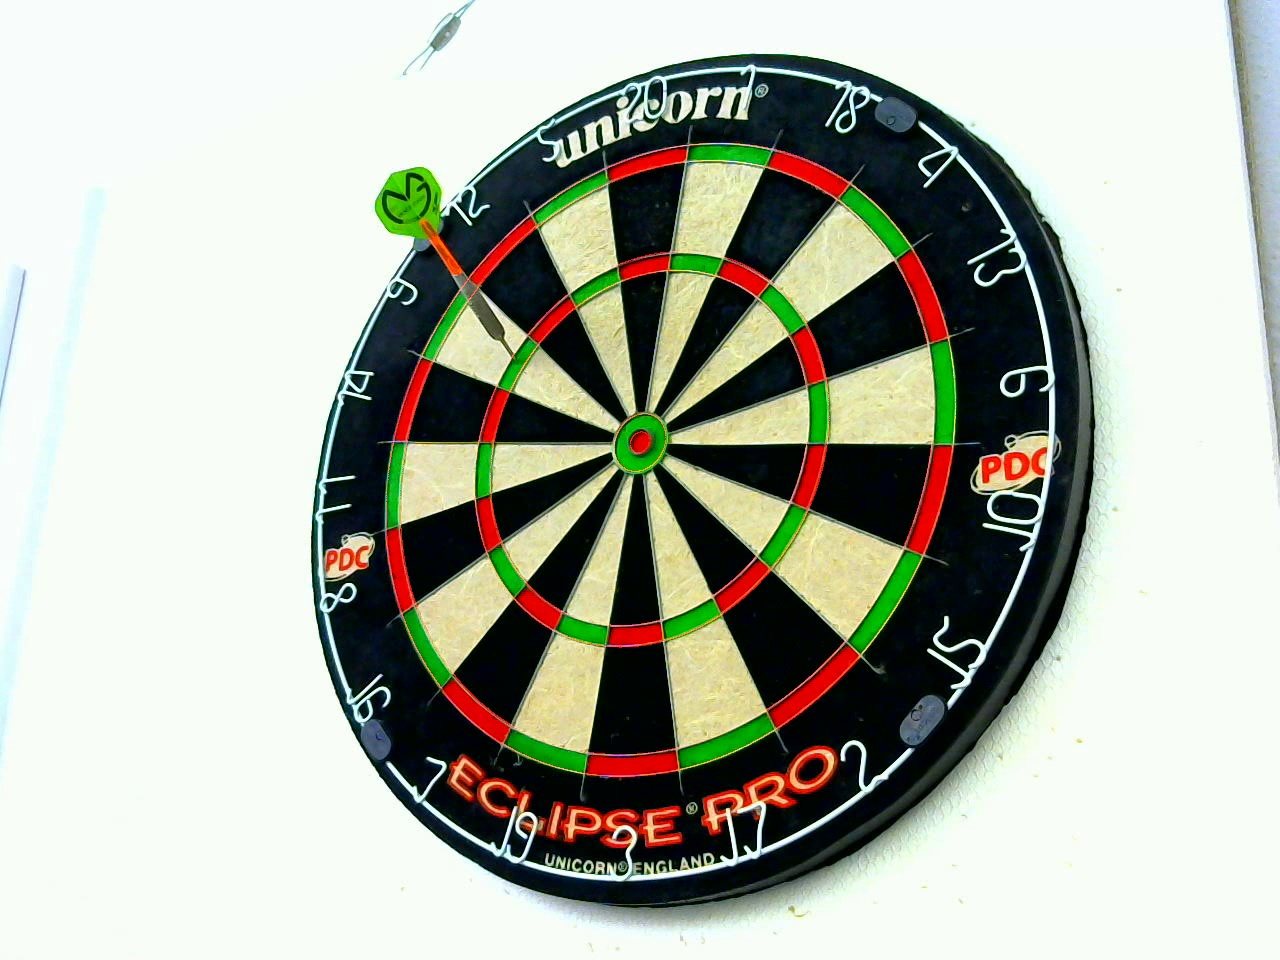
\includegraphics[width=0.48\textwidth]{media/current}}\\
\begin{center}
\subfloat[Vordergrund-Maske]{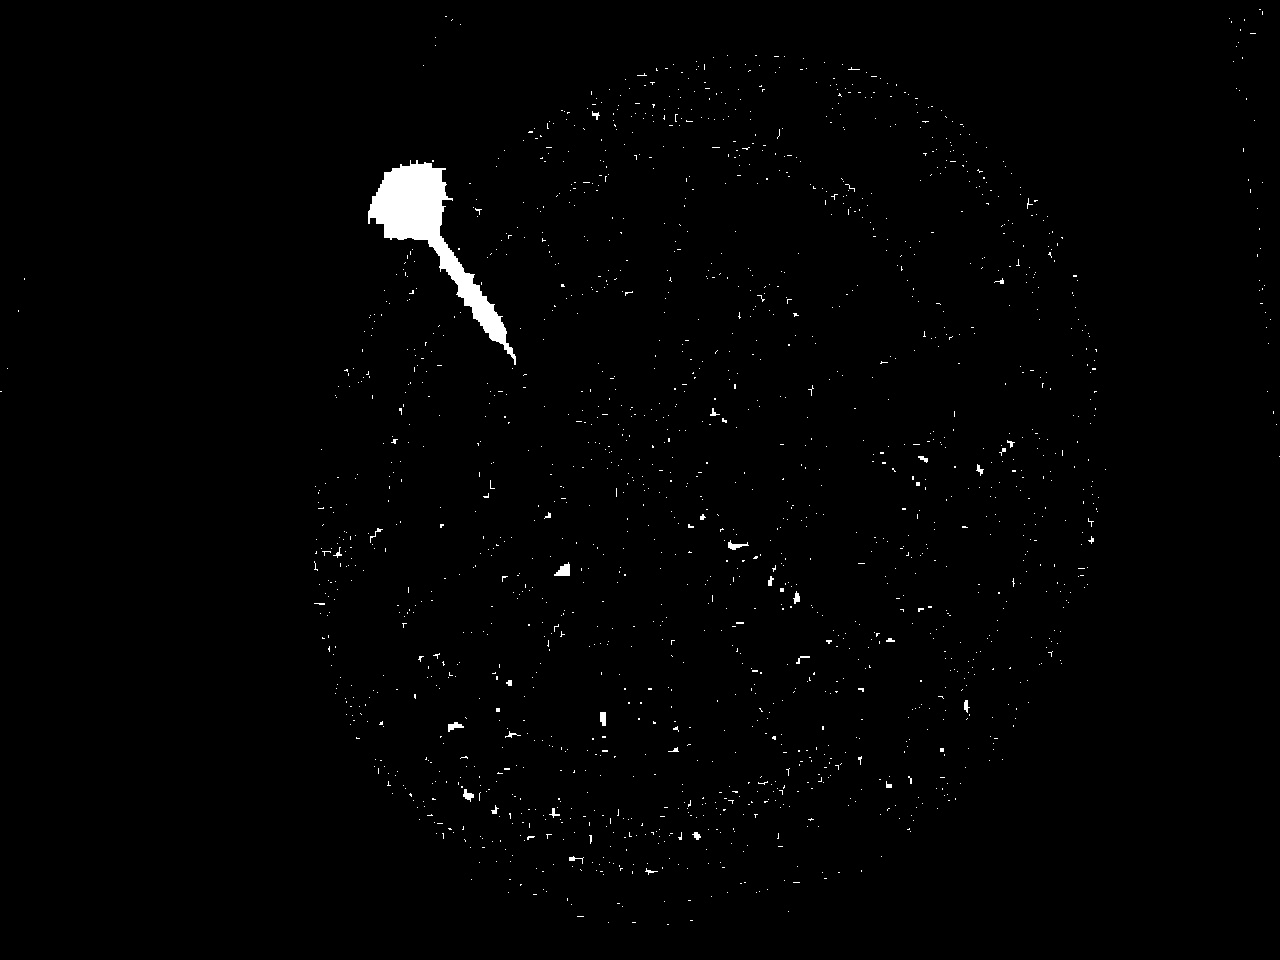
\includegraphics[width=0.48\textwidth]{media/substracted}}
\par\end{center}
\caption{\textbf{Grundvorgehen Background-Substraction}}
\label{Fig:background}
\end{figure}

Ein naiver Ansatz wäre Beispielsweise ein Bild zu setzen, das als Hintergrund gewählt werden soll und in Schritt 2 eine einfache Differenz zwischen Hintergrund und Bild zu berechnen. Anschließen könnte man ein Thresholding betreiben und alle Pixel auswählen die eine Differenz aufweisen, die höher als der Schwellwert ist. \autocite[3]{foreground2003}
Diese werden dann in das Binär Bild, der Maske übertragen. 

Dieser naive Ansatz ist allerdings anfällig gegen Beispielsweise sich verändernde Lichtverhältnisse. Aus dem Grund der Anfälligkeit werden andere Modellierungen gewählt. Eine der beliebtesten und meist verbreitetsten ist ein Iterativer Ansatz, genauer Mixture of Gaussians (MoG). Hierbei wird das Modell regelmäßig aktualisiert, sodass langsame Veränderungen im Bild in es einfließen. \autocite[4]{foreground2003}

In OpenCV sind verschiedene Varianten von Background-Substractoren implementiert. Unter anderen auch zwei Versionen des MoG \autocite{OpenCVBack2016}. Im folgenden ein kurzer Überblick, über genutzte Funktionen:
\begin{lstlisting}[frame=single,language=Python]
substractor = createBackgroundSubtractorMOG2()
fgmask = substractor.apply(image)
\end{lstlisting}
Dabei initiiert die erste den Substractor.
Mit \textit{apply(image)} wird der Substractor mit Bildern gespeist. Diese bilden dann intern das Hintergrundmodell. Ebenfalls wird mit dieser Funktion der Hintergrund subtrahiert und es wird die entsprechende Vordergrund-Maske zurückgegeben. 
Der Substractor hat einige Parameter anhand derer man die Funktionalität abstimmen kann und auf das gegebene Szenario anpassen kann. Einige der wichtigsten sind:
\begin{itemize}
	\item \textbf{history:} Die Anzahl der Bilder, die in das Hintergrund-Modell einfließen
	\item \textbf{detectShadows:} Gibt an ob Schatten erkannt werden sollen und als Graustufen in die Vordergrund-Maske einfließen
	\item \textbf{varThreshold:} Der Threshold der die Masken-Bildung steuert
	\item \textbf{shadowThreshold:} gibt den Treshold an bei dem ein Schatten erkannt werden soll
\end{itemize}
Dabei ist die Größe der History stark von den Frames per second (FPS) des eingehenden Bilder-Streams abhängig, zudem vom eigentlichen Szenario. In dem hier betrachteten Fall treffen die Darts auf dem Dartboard auf und verändern anschließend ihre Position nicht mehr. Hinzu kommt, dass die Darts in schneller Abfolge geworfen werden können und auf das Board auftreffen. Aus diesem Grund sollte als History ein Wert gewählt werden, der wenigen Sekunden entsprechend der Video-Stream FPS entsprechen. Wenn bei $30FPS$ das Hintergrund-Modell aus den letzten 4 Sekunden erstellt werden soll, so ergibt sich: $30FPS * 4 Sekunden = 120 Frames$.
Zu den beiden prozentualen Threshold-Werten gibt es jeweils noch Maximum und Minimum Werte die gesetzt werden können, um das Ergebnis zu beeinflussen.

Das Ergebnis dieser Vordergrund-Erkennung ist ein Binär-Bild, das die Regionen im Bild aufzeigt die potentiell zum Vordergrund gehören. Im folgenden muss entschieden werden, welche Regionen als Dart erkannt werden sollen. Dieses Binär-Bild wird dem Contour-Storage übergeben und weiter verarbeitet. Der beschriebene Vorgang ist in den grau hinterlegten Bereich in der Pipeline-Übersicht in Abbildung\prettyref{Fig:pipeline} einzuordnen und wird laufend für jedes eintreffende Bild wiederholt.



\section{Blob Erfassung}
\label{sec:blob}

\begin{itemize}
\item Bilder der Plots für Blob größe
\item Beschreiben wie die neue Maske aus dem Blob aufgebaut wird
\item Vorteile und Grund hierfür erläutern
\item Resultat eine weitere Maske 
\end{itemize}

Werden die Binär-Bilder dem Storage hinzugefügt, werden einige Parameter bestimmt, die dem neuen Eintrag hinzugefügt werden.
Einer dieser Einträge enthält dann Informationen:
\begin{enumerate}
	\item Das Binär-Bild der Vordergrund-Maske
	\item Anzahl Blobs über einem Threshold
	\item Größe des größten Blobs
\end{enumerate}
Dabei werden der zweite und dritte Parameter bestimmt, indem auf dem Binär-Bild Gruppen von zusammenhängenden Pixeln (Blobs) erkannt werden. 
Grundlegend wird dabei die Nachbarschaft, der weißen Pixel betrachtet. Zusammenhängende werden einem Blob zugeordnet. Auch an dieser Stelle wird auf bereitgestellte OpenCV Funktionen zurückgegriffen. Dem Eintrag wird nun die Anzahl der Pixel, des größten zusammenhängenden Blobs hinzugefügt. Zudem werden alle Blobs ausgeschlossen, die eine bestimmte Größe unterschreiten. Dadurch wird verhindert, dass Rauschen in späteren Schritten eine weiter Verarbeitung auslöst und so unnötigen Overhead verursacht.
\begin{figure}[ht]
\centering
\subfloat[]{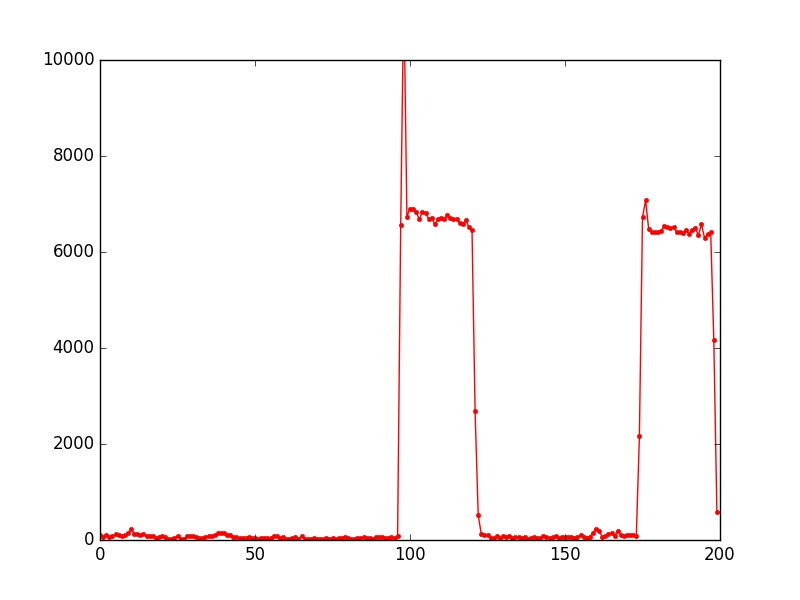
\includegraphics[width=0.9\textwidth]{media/plot.jpg}}\qquad
\caption{\textbf{Plot des Storages}}
\label{Fig:blobplot}
\end{figure}

Der Storage hat eine gewissen Größe und speichert die Bilder und Information. Der Storage ist als Queue entworfen. Wenn also Einträge entsprechend der Größe der Queue hinzugefügt wurden, werden die vorderen Einträge entfernt. In Abbildung \prettyref{Fig:blobplot} ist die Anzahl der Pixel des größten Blobs, den Einträgen im Verlauf gegenübergestellt.

Nun soll im Storage ein Interessanter Bereich entdeckt werden, in dem ein Dart im Bild erkannt werden könnte. Die Grundidee ist, dass ein Dart mindestens eine gewissen Pixel-Anzahl im Bild einnimmt. Abhängig von der Background-Substraction kann Anzahl der Einträge in denen der Dart sichtbar ist variieren. So ist ein Bereich von Interesse, wenn die Anzahl an zusammenhängenden Pixeln größer ist als die vermutliche Anzahl die ein Dart einnimmt.

Um einen Bereich zu bestimmen werden nun zusammenhängende Bereiche gesucht. Hierfür wird erst ein Startpunkt ermittelt und ausgehend von diesem der passende Endpunkt.
Ab Eintrag 98 ist ein starker Anstieg zu erkennen. Steigen die Werte über einen gewissen Threshold wird der Start eines Abschnittes markiert. Das Ende eines Abschnittes wird markiert, wenn die Blob-Größe für eine gewisse Dauer unter dem Threshold liegt. Im abgebildeten Plot ist der Endpunkt an Eintrag 120 erreicht. Somit ist der Bereich von 98 bis 120 von Interesse und wird für weitere Verarbeitung genutzt. 
Wenn die Länge, der zusammenhängenden Bereiche unter einer Mindestlänge liegt werden diese ignoriert.

An dieser Stelle wird noch eine weitere wichtige Funktion erfüllt. Es wird bereits eine erste Sondierung vorgenommen, welche Bilder und Storage-Bereiche nicht verwertbar sind. 
Ein spezielles Beispiel ist dabei, dass die Darts wieder aus dem Dartboard entfernt werden müssen. Hierbei greift der Nutzer in Bildbereich und verursacht dadurch einen sehr großen Bereich in der Vordergrund-Maske dieser verursacht großen overhead und wird daher aus der Berechnung entfernt. Zu diesem Zweck wird nicht nur ein Mindestschwellwert gesetzt, sondern auch ein Höchstschwellwert. Wird dieser prozentual gesehen zu der Bildgröße überschritten, wird für einige Sekunden das Erstellen neuer Einträge in den Storage geblockt.

In einem weiteren Schritt werden die Bilder aus diesem Bereich analysiert und es wird ein neues Binär-Bild daraus erstellt. Dieses neue Bild fasst die Informationen von allen Bildern in dem Storage-Bereich zusammen und bildet diese ab.
Das Vorgehen dabei ist in drei Schritte unterteilt.
Im ersten Schritt wird ein Graustufen-Bild erstellt, in dem initial alle Pixel schwarz sind. 
Im zweiten Schritt wird über die Bilder des Storage-Bereiches iteriert. Dabei wird für jeden weißen Pixel des Bildes im neuen Graustufen-Bild der entsprechende Pixel um einen gewissen Wert erhöht. Welcher Wert auf die Pixel addiert wird ist abhängig von der History-Größe des Background-Substractors.
\begin{figure}[ht]
\centering
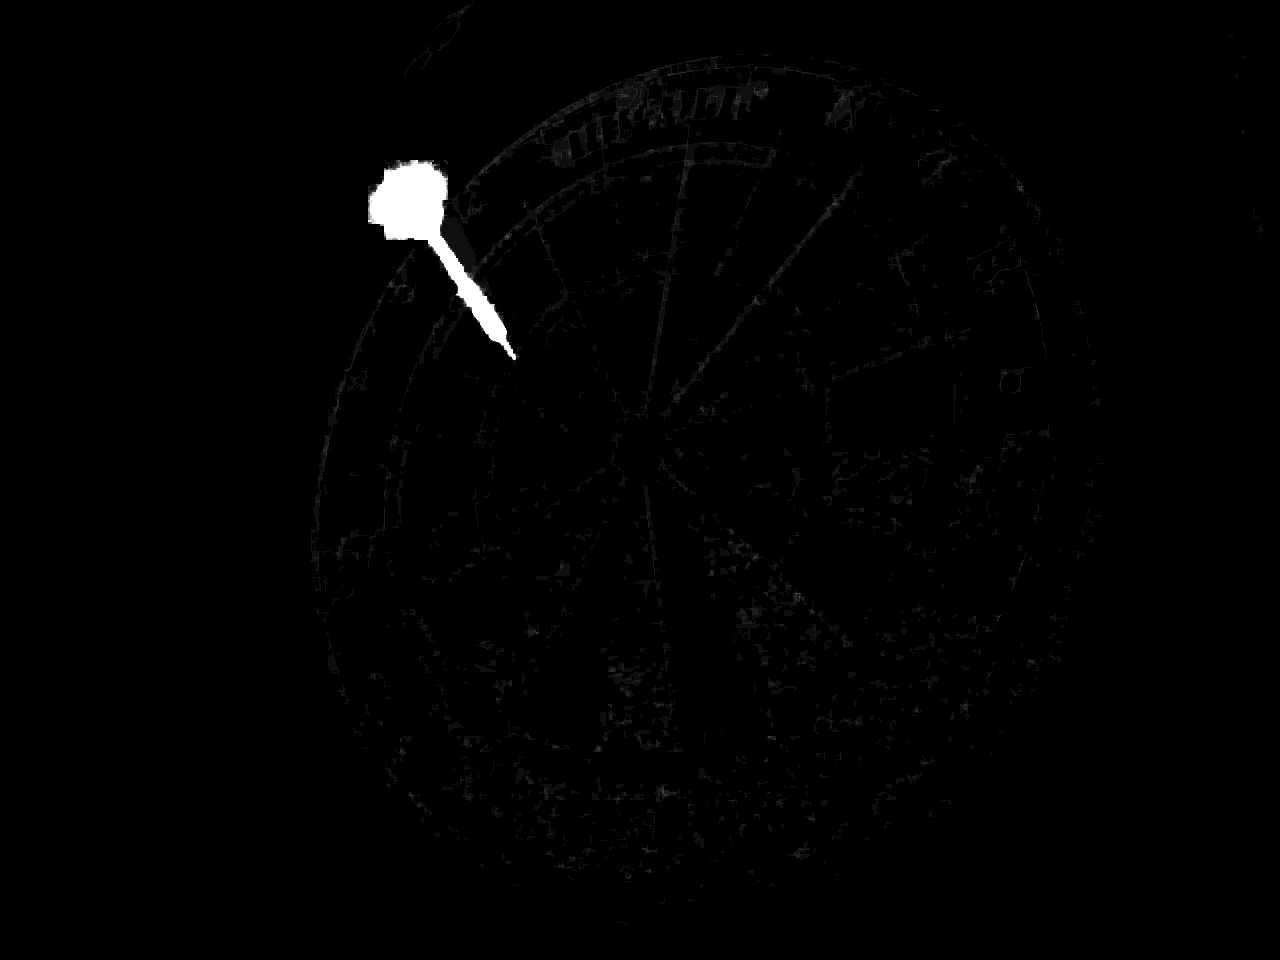
\includegraphics[width=0.9\textwidth]{media/blobimg}
\caption{\textbf{Resultierendes Graustufen Bild}}
\label{Fig:greyimg}
\end{figure}
Ist das Graustufen-Bild gebildet, ein Beispiel ist in Abbildung \prettyref{Fig:greyimg} zu sehen, kann dieses im dritten Schritt verarbeitet werden. 
Im letzten Schritt wird das Graustufen-Bild in ein Binär-Bild gewandelt und dabei ein Thresholding angewendet. So sind in dem resultierenden Bild nur die Regionen zu sehen, die in einem Großteil des Storage-Bereiches auftreten. 

Dieses Vorgehen hat mehrere Gründe. 
Zum einen kann so Rauschen aus einigen wenigen Bildern gemildert werden. 
Ein weiterer Grund ist, dass auf diese Weise ein klarerer Umriss erstellt werden kann, aus dem später der Dart erkannt werden kann. 
Dieser Vorgang ist der erste Part des in Abbildung \prettyref{Fig:pipeline} blau markierten Bereiches und der erste Schritt zur Punktzahlbestimmung aus den gelieferten Bildern. Das resultierende Binär-Bild wird von der Kontur Erkennung weiter verarbeitet.

\section{Verarbeitung der Vordergrundinformationen}
\label{sec:foreground}
%Stage 4 Im Extrahierten Vordergrund entscheiden was Pfeil ist
%\begin{itemize}
%\item Kontur erkennen
%\item Momente der Kontur erkennen
%\item Aus den Momenten die Spitze der Darts erkennen
%\item die 5 Arten der Spitze erläutern
%\end{itemize}
Im errechneten Vordergrund gilt es nun den Dart zu erkennen und die Spitze des Darts zu bestimmen. Grundsätzlich gibt es die Möglichkeit Objekte anhand der Farbgebung Objekte auszumachen. Da beim Dartsport keine Standardisierung für einheitliche Farbgebung der Darts gegeben ist, gibt es diese Möglichkeit nicht. Aus diesem Grund müssen die Darts aufgrund ihrer Form erkannt werden. In einem 2D-Bild entspricht das der Kontur.
\begin{figure}[ht]
\centering
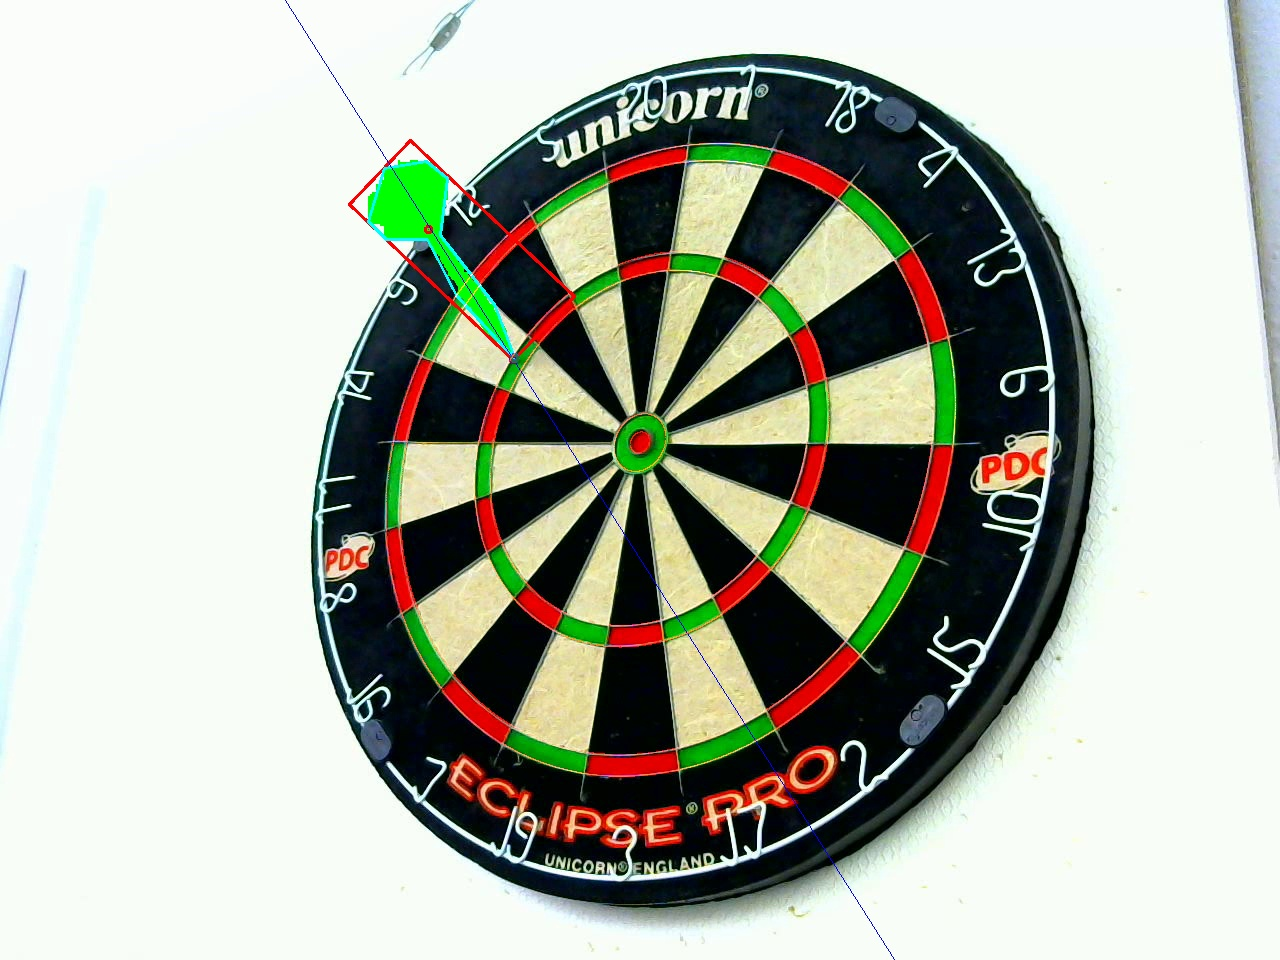
\includegraphics[width=0.9\textwidth]{media/backgroundfeature}
\caption{\textbf{Ein Dart mit eingezeichneten Momenten und Spitzen}}
\label{Fig:detecteddart}
\end{figure}
Bereits 1985 gab es Forschungen Konturen in Binär-Bildern zu erkennen. Satoshi Suzuki hat einen Artikel veröffentlicht in dem ein solcher Algorithmus präsentiert wird \autocite{contour1985}. Dieser Algorithmus ist ebenfalls in OpenCV implementiert. 

Nun kann das aus der Bereichserkennung stammende Bild in die Kontur-Erkennung von OpenCV übergeben werden. Auf den erkannten Konturen können dann weitere Charakteristika (Features) bestimmt werden. Einige der genutzten und wichtigsten sind:
\begin{itemize}
	\item \textbf{Eingrenzendes Rechteck (Bounding Rectangle)} Kleinstmögliches Rechteck, das die Kontur umschließt
	\item \textbf{Linie durch Kontur}
	\item \textbf{Schwerpunkt (Centroid)} 
	\item \textbf{approximierte Kontur} Eine Approximierte Kontur, deren maximale Abweichung zur Ausgangs-Kontur in einem bestimmten Threshold liegt.
\end{itemize}
Diese Charakteristika werden genutzt, um zu bestimmen ob eine Kontur ein Dart sein kann und wo dessen Spitze liegt. Zur Bestimmung der genannten Features werden vorhandene OpenCV Funktionen genutzt. Unter anderen folgende:
\begin{lstlisting}[frame=single]
contours,hierarchy = findContours(image, mode, method)
rect = minAreaRect(contour)
M = moments(contour)
vector = fitLine(contour)
\end{lstlisting}
Dabei können der Funktion zur Kontur-Erkennung auf einem Binär-Bild noch ein Modus und eine Methode übergeben werden. Der Modus definiert, ob nur die äußersten Konturen zurückgegeben werden sollen, oder eine hierarchische Struktur aufgebaut werden soll. In unserem Fall ist nur die äußere Kontur des Darts von Interesse. Mit der Methode kann bestimmt werden, ob eine Approximation der Kontur stattfinden soll. So könnte bei einer rechteckigen Kontur diese Beispielsweise auf die Eckpunkte reduziert werden. Finde keine Approximation statt werden alle Punkte entlang der Kanten zurück gegeben. Von dieser Methode wird dann eine Liste an möglichen Konturen zurückgegeben. 

Auf diesen Konturen werden anschließen die genannten Features berechnet.
Zudem werden die errechneten Charakteristika später für die Erkennung der Spitze genutzt.
Sind folgende Bedingungen gegeben wird die Kontur als Dart gewertet und es wird versucht eine Spitze zu erkennen:
\begin{itemize}
	\item Größe des umschließenden Rechteckes
	\item Seitenverhältnis des umschließenden Rechteckes
	\item Größe der Kontur
	\item Centroid der Kontur ist in einem Mindestabstand zum Centroid des umschließenden Rechteckes. Dies tritt auf, da der Flight des Darts den Centroid der Kontur stark in die entgegengesetzte Richtung der Spitze verschiebt. 
\end{itemize}

Die Kontur und die errechneten Features können nun in den Schritt zur Erkennung der Dart-Spitzen übergeben werden.


\section{Punktzahlbestimmung}
\label{sec:score}
Zur Bestimmung der Punktzahl fließen nun bisher erlangte Informationen aus der Verarbeitung des Vordergrundes \prettyref{sec:foreground} und Informationen zum Dartboard \prettyref{sec:board} zusammen.
So wird aus der Kontur und den zugehörigen Features die Spitze des Darts errechnet. Ist der Pixel der Spitze errechnet, kann mit Hilfe der Transformationsmatritzen der zugehörige Punkt im Modell des Dartboardes errechnet werden. Ist der Punkt errechnet kann aus dem Modell die Punktzahl des Feldes ermittelt werden. 

\begin{figure}[ht]
\centering
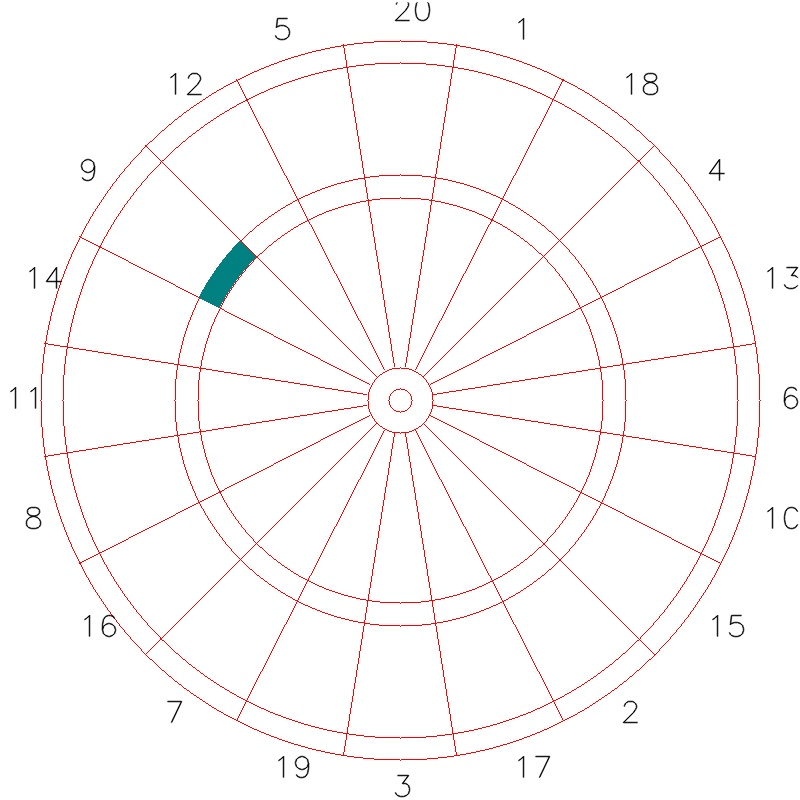
\includegraphics[width=0.39\textwidth]{media/pointimg}
\caption{\textbf{Markierung des getroffenen Feldes}}
\label{Fig:acceptingimg}
\end{figure}

Insgesamt wurden fünf verschiedene Varianten zu Bestimmung der Spitze der Darts durchgeführt. 
\begin{enumerate}
	\item Der Punkt auf der Kontur, der die höchste Distanz zum Centroid aufweist
	\item Der Punkt, an dem die Linie durch die Kontur das umschließenden Rechteck schneidet. Aus den zwei resultierenden Punkten wird der gewählt, der die größere Distanz zum Centroid aufweist.
	\item Der Punkt auf der approximierten Kontur, der die höchste Distanz zum Centroid  aufweist
	\item Der Punkt an dem die approximierten Kontur die umschließende Box berührt und die höchste Distanz zum Centroid aufweist
	\item Der Schwerpunkt, der vorigen vier Ansätze
\end{enumerate}

Für jeden dieser so bestimmten Punkte wird anschließend eine Transformation ein das Modell Koordinatensystem durchgeführt. \todo{Formel der inversen Aufzeigen.}
Sind Punkt im Modell bestimmt und das zugehörige Feld des Dartboards bestimmt, wird das Ergebnis aller fünf möglichen Spitzen gespeichert. Zur Überprüfung wird der Nutzer gebeten zu bestätigen, welches Feld tatsächlich getroffen wurde. 

In Abbildung \prettyref{Fig:acceptingimg} wird dargestellt, wie dem Nutzer vermittelt wird, welches Feld getroffen wurde. Zudem kann an dieser Stelle eine Bestätigung statfinden, indem das tatsächlich getroffene Feld angeklickt wird.


